\subsection{Nomenclature}
A transfer line is a production system where the machines in series may or not be separated by buffers, to form a unidirectional graph. An example for a production graph can be found in figure \ref{fig:simple_transfer_line}. 
The machines were indicated by a square and a buffer with a circle and their corresponding parameters are listed in table \ref{tab:module_parameters} and table \ref*{tab:buffer_parameters}.

\begin{figure}[htbp]
    \centering
    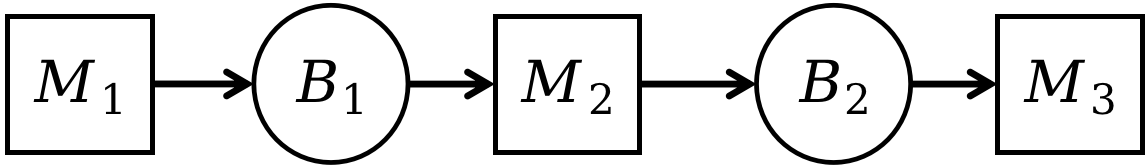
\includegraphics[width=0.4\textwidth]{figures/transfer_line.png} 
    \caption{Three machine transfer line}
    \label{fig:simple_transfer_line}
\end{figure}

\begin{table}[htbp]
    \begin{minipage}{0.5\linewidth}
        \centering
        \begin{tabular}{|c|p{4cm}|}
            \hline
            \parbox[c]{2cm}{\centering 
\includegraphics[width=1cm]{figures/module.png}} & Machine or module to carry operation.\\
            \hline  
            $\mu_{m} = 1 / cycle time $ &  Processing rate\\
            \hline
            $MTTF$ & Mean Time To Fail\\
            \hline
            $MTTR$ & Mean Time To Repair\\
            \hline
        \end{tabular}
        \caption{Module parameters}
        \label{tab:module_parameters}
    \end{minipage}%
    \begin{minipage}{0.5\linewidth}
        \centering
        \begin{tabular}{|c|p{4cm}|}
            \hline
            \parbox[c]{2cm}{\centering 
\includegraphics[width = 1cm]{figures/buffer}} & Buffer to store parts in between operations.  \\
            \hline
            $N \lbrace b \rbrace $& Maximum buffer capacity \\
            \hline
            $L \lbrace b \rbrace$ & Minimum buffer capacity \\
            \hline
        \end{tabular}
        \caption{Buffer Parameters}
        \label{tab:buffer_parameters}
    \end{minipage}
\end{table}

\textbf{Processing rate ($\mu_m$):} The amout of material can be operated on the machine in a unit time. \par
\textbf{Meantime to fail (MTTF):} As the name defines, it's a statistical representation of a distribution that can be used to generate the random variable that gives the operation time before its next failure.\par
\textbf{Meantime to repair (MTTR):} Similar to MTTF, it's a statistical representation of a distribution that gives a number to indicate the time required to repair a machine.\par
\textbf{Buffer capacity ($N \lbrace b  \rbrace$):} It's a limit to number of parts can be stored in buffer at a given time.